\documentclass[aspectratio=169]{beamer}

\usetheme{GRVC}

% Blocks
\setbeamerfont{block title}{size=\normalsize, series=\bfseries}
\setbeamerfont{block body}{size=\small}

% Itemize / enumerate
\setbeamerfont{itemize/enumerate body}{size=\small}
\setbeamerfont{itemize/enumerate subbody}{size=\footnotesize}


\usepackage{tikz}
\usetikzlibrary{calc}

% Partner logo helper (used for consortium slides)
\newcommand{\GRVCpartnerlogo}[1]{%
  \includegraphics[width=0.16\textwidth,height=1.5cm,keepaspectratio]{#1}%
}

% Set a transparent background image for all frames
\setbeamertemplate{background}{%
  \begin{tikzpicture}[remember picture,overlay]
    \node[opacity=0.95, at=(current page.center)] {%
      \includegraphics[width=\paperwidth,height=\paperheight]{assets/background.png}%
    };
  \end{tikzpicture}%
}

\title{GRVC Lab\\Biweekly seminars}
\author{Abdalraheem Abdullah Yousef Ijieh}
% \institute{GRVC Robotics Labs}
\date{16 Enero 2026}

\begin{document}

% Title slide (first slide) includes GRVC logo at lower-left by design
\begin{frame}[plain]
  \titlepage
\end{frame}


% Example: section divider with project logo (top-right)
\GRVCsectionframe[assets/tema\_logo.png]{Trusted extremely precise mapping and prediction for emergency management}

% --- Consortium partners (logos are sourced from the official TEMA partners page) ---
{\setbeamertemplate{background}{%
  \begin{tikzpicture}[remember picture,overlay]
    \fill[GRVCCYAN] (current page.south west) rectangle (current page.north east);
  \end{tikzpicture}}
  }


{
\GRVCsetprojectlogo{assets/tema_logo.pdf}
\begin{frame}{TEMA in a Nutshell}
  \begin{columns}[T,onlytextwidth]
    % ---------------- Left column: Partners ----------------
    \column{0.4\textwidth}
      \centering
      {\bfseries Consortium partners}\par\vspace{0.4em}

      % tighten spacing so it fits nicely
      \setlength{\tabcolsep}{3pt}
      \renewcommand{\arraystretch}{0.95}

      \begin{tabular}{ccccc}
        \GRVCpartnerlogo{assets/partners/auth.png} &
        \GRVCpartnerlogo{assets/partners/atos.png} &
        \GRVCpartnerlogo{assets/partners/brk.png} &
        \GRVCpartnerlogo{assets/partners/dmalian.png} &
        \GRVCpartnerlogo{assets/partners/engineering.png} \\
        \GRVCpartnerlogo{assets/partners/fraunhofer_hhi.png} &
        \GRVCpartnerlogo{assets/partners/dlr.png} &
        \GRVCpartnerlogo{assets/partners/itu.png} &
        \GRVCpartnerlogo{assets/partners/kamk.png} &
        \GRVCpartnerlogo{assets/partners/kaj.png} \\
        \GRVCpartnerlogo{assets/partners/kemea.png} &
        \GRVCpartnerlogo{assets/partners/latitudo40.png} &
        \GRVCpartnerlogo{assets/partners/nelen_schuurmans.png} &
        \GRVCpartnerlogo{assets/partners/northdocks.png} &
        \GRVCpartnerlogo{assets/partners/plus.png} \\
        \GRVCpartnerlogo{assets/partners/ras.png} &
        \GRVCpartnerlogo{assets/partners/tecnosylva.png} &
        \GRVCpartnerlogo{assets/partners/lisbon_council.png} &
        \GRVCpartnerlogo{assets/partners/use.png} &
        \GRVCpartnerlogo{assets/partners/unime.png} \\
      \end{tabular}

    % ---------------- Right column: At a glance ----------------
    \column{0.54\textwidth}
    \centering 
    {\bfseries \large TEMA at a glance}\par\vspace{0.3em}
    \centering
    \begin{tabular}{ccc}
      {20 Partners} & {4 Years} & {11 M\texteuro}
    \end{tabular}
    \par\vspace{0.7em}
    \raggedright

    % Optional: also shrink block title/body a touch (local to this frame/column)
    \setbeamerfont{block title}{size=\footnotesize,series=\bfseries}
    \setbeamerfont{block body}{size=\scriptsize}
    \setbeamerfont{itemize/enumerate body}{size=\scriptsize}

    \begin{block}{Mission}
      Deliver actionable situational awareness for disaster response by turning multi-source data into decision-ready information.
    \end{block}

    \vspace{-0.3em}
    \begin{itemize}
      \setlength{\itemsep}{0.35em}
      \item Bring real-time situational data to responders and relevant end-users.
      \item Support operational decision-making during evolving incidents.
      \item Transferable across hazards (e.g., flood, wildfire) and geographic regions.
    \end{itemize}

  \end{columns}
\end{frame}
\GRVCclearprojectlogo
}

%%%%%%%%%%%%%%%%%%%%%%%%%%%%%%%%%%%%%%%%%%%%%%%
% --- TEMA technologies (USE highlighted) ---
{
\GRVCsetprojectlogo{assets/tema_logo.pdf}

% Robust highlighting (avoid table-row coloring issues on beamer themes)
\newcommand{\USEtech}[1]{\textbf{\textcolor{GRVCCyan}{#1}}}

\begin{frame}{TEMA technologies}
  \scriptsize
  \setlength{\tabcolsep}{2pt}
  \renewcommand{\arraystretch}{0.95}
  \tiny
  \begin{columns}[T,onlytextwidth]
    % ---------------- TFA ----------------
    \column{0.4\textwidth}
    {\bfseries Trustworthy Federated Analytics}\par\vspace{0.25em}
    \begin{tabular}{@{}p{0.24\linewidth}p{0.74\linewidth}@{}}
      \textbf{ID} & \textbf{Technology}\\ \hline
      TFA-tech-01 & Concept discovery for latent space interpretability of deep neural networks\\
      TFA-tech-02 & Human-comprehensible presentation of concept-based explanations\\
      TFA-tech-03 & DNN robustness\\
      TFA-tech-04 & Explainability for transformer base neural networks\\
      TFA-tech-05 & Fire/smoke/flood/person detection\\
      TFA-tech-06 & Fire/flood/background segmentation\\
      TFA-tech-07 & Person re-identification\\
      TFA-tech-08 & Satellite-based flood detection and assessment\\
      TFA-tech-09 & Satellite-based Forest fire detection and assessment\\
      TFA-tech-10 & Privacy preservation during visual analysis\\
      TFA-tech-11 & Geo-social media analysis\\
      TFA-tech-12 & Sentiment analysis for short texts\\
      TFA-tech-13 & Contrastive image-language models\\
      TFA-tech-14 & Federated Learning\\
      TFA-tech-15 & Data scarcity, synthetic data generation pipeline\\
    \end{tabular}

    % ---------------- PDM ----------------
    \column{0.29\textwidth}
    {\bfseries Phenomenon Prediction and Decision-Macking}\par\vspace{0.25em}
    \begin{tabular}{@{}p{0.44\linewidth}p{0.54\linewidth}@{}}
      \textbf{ID} & \textbf{Technology}\\ \hline
      PDM-tech-01 & Forest Fire Simulation\\
      PDM-tech-02 & 3Di Hydrodynamic simulation\\
      PDM-tech-03 & Realistic 3D smoke modelling and fire detection\\
      \USEtech{PDM-tech-04} & \USEtech{Drone planning}\\
      \USEtech{PDM-tech-05} & \USEtech{Information fusion}\\
      PDM-tech-06 & Data-fusion-based decision support and process triggering\\
    \end{tabular}

    % ---------------- SV ----------------
    \column{0.24\textwidth}
    {\bfseries Simulation and Visualization}\par\vspace{0.25em}
    \begin{tabular}{@{}p{0.44\linewidth}p{0.54\linewidth}@{}}
      \textbf{ID} & \textbf{Technology}\\ \hline
      \USEtech{SV-tech-01} & \USEtech{Drone-based image and data acquisition}\\
      SV-tech-02 & Digital Enabler\\
      SV-tech-03 & 3D computer vision (SfM)/ Photogrammetry\\
      SV-tech-04 & Geovisual Analytics\\
      SV-tech-05 & Geospatial information retrieval\\
      SV-tech-06 & Extended Reality-based interactive visualisation system\\
      SV-tech-07 & Smartdesk\\
    \end{tabular}
  \end{columns}

  \vspace{0.4em}
  \tiny \textcolor{GRVCCyan}{\rule{0.9em}{0.9em}} \; \textit{University of Seville (USE) technologies: SV-tech-01, PDM-tech-04, PDM-tech-05.}
\end{frame}
\GRVCclearprojectlogo
}

% ------------------------------------------------------------
% Information Fusion (PDM-tech-05) — University of Seville (USE)
% ------------------------------------------------------------
\GRVCsectionframe[assets/tema\_logo.png]{Information fusion (PDM-tech-05)}

{
\GRVCsetprojectlogo{assets/tema_logo.pdf}
}

% Clean background for technical content (better readability than a photo background)
%\setbeamertemplate{background}{%
%  \begin{tikzpicture}[remember picture,overlay]
%    \fill[GRVCBlue] (current page.south west) rectangle (current page.north east);
%  \end{tikzpicture}%
%}

%\begin{frame}[t]{Information fusion: storyline}
%	\small
%	\setlength{\itemsep}{0.25em}
%	\setlength{\topsep}{0.2em}
%	
%	\begin{itemize}
%		\item Operational problem: multi-source data $\rightarrow$ fragmented situational awareness
%		\item Platform concept: a generic fusion service for natural-disaster management (floods, fires, \dots)
%		\item System integration: from sensors and models to the TEMA Digital Enabler / SmartDesk
%		\item Output products:
%		\begin{itemize}
%			\setlength{\itemsep}{0.15em}
%			\setlength{\topsep}{0.1em}
%			\item \textbf{OGM}: disaster status (flood / fire) on a common grid
%			\item \textbf{OPM}: multi-object tracking (persons / vehicles) in geodetic space
%		\end{itemize}
%		\item Fusion methods: asynchronous Bayesian updates + model-aware prediction pooling
%		\item Case study: flood scenario (Ahrtal) demonstrating end-to-end behaviour
%	\end{itemize}
%\end{frame}


\begin{frame}[t]{Motivation and end-to-end workflow in TEMA}
	
	\footnotesize
	\setlength{\itemsep}{0.2em}
	\setlength{\topsep}{0.2em}
	
	\begin{block}{Why we need information fusion}
		In an evolving disaster, decisions are time-critical and data are imperfect.
		Sensors and models provide partial, asynchronous, and uncertain evidence.
		The command centre needs a single, continuously updated operational picture.
	\end{block}
	
	\vspace{0.4em}
	
	\begin{columns}[T,onlytextwidth]
		% -------- Left: text (two mini-columns) --------
		\begin{column}{0.60\textwidth}
			\begin{columns}[T,onlytextwidth]
				\begin{column}{0.50\textwidth}
					\textbf{Typical inputs}
					\tiny
					\begin{itemize}
						\tiny
						\setlength{\itemsep}{0.15em}
						\setlength{\topsep}{0.1em}
						\setlength{\parskip}{0pt}
						\item UAV imagery (flood/fire segmentation; person/vehicle detection)
						\item Satellite products (medium-resolution, large coverage)
						\item Simulations (hydrodynamic depth, fire spread / arrival time)
						\item Geosocial media analysis
					\end{itemize}
				\end{column}
				
				\begin{column}{0.50\textwidth}
					\footnotesize
					\textbf{Operational questions}					
					\begin{itemize}
						\tiny
						\setlength{\itemsep}{0.15em}
						\setlength{\topsep}{0.1em}
						\setlength{\parskip}{0pt}
						\item Where is the hazard now (and how confident are we)?
						\item Where will it be next (and when)?
						\item Where are people / vehicles at risk?
						\item Which areas should drones revisit?
					\end{itemize}
				\end{column}
			\end{columns}
		\end{column}
		
		% -------- Right: figure --------
		\begin{column}{0.40\textwidth}
			\centering
			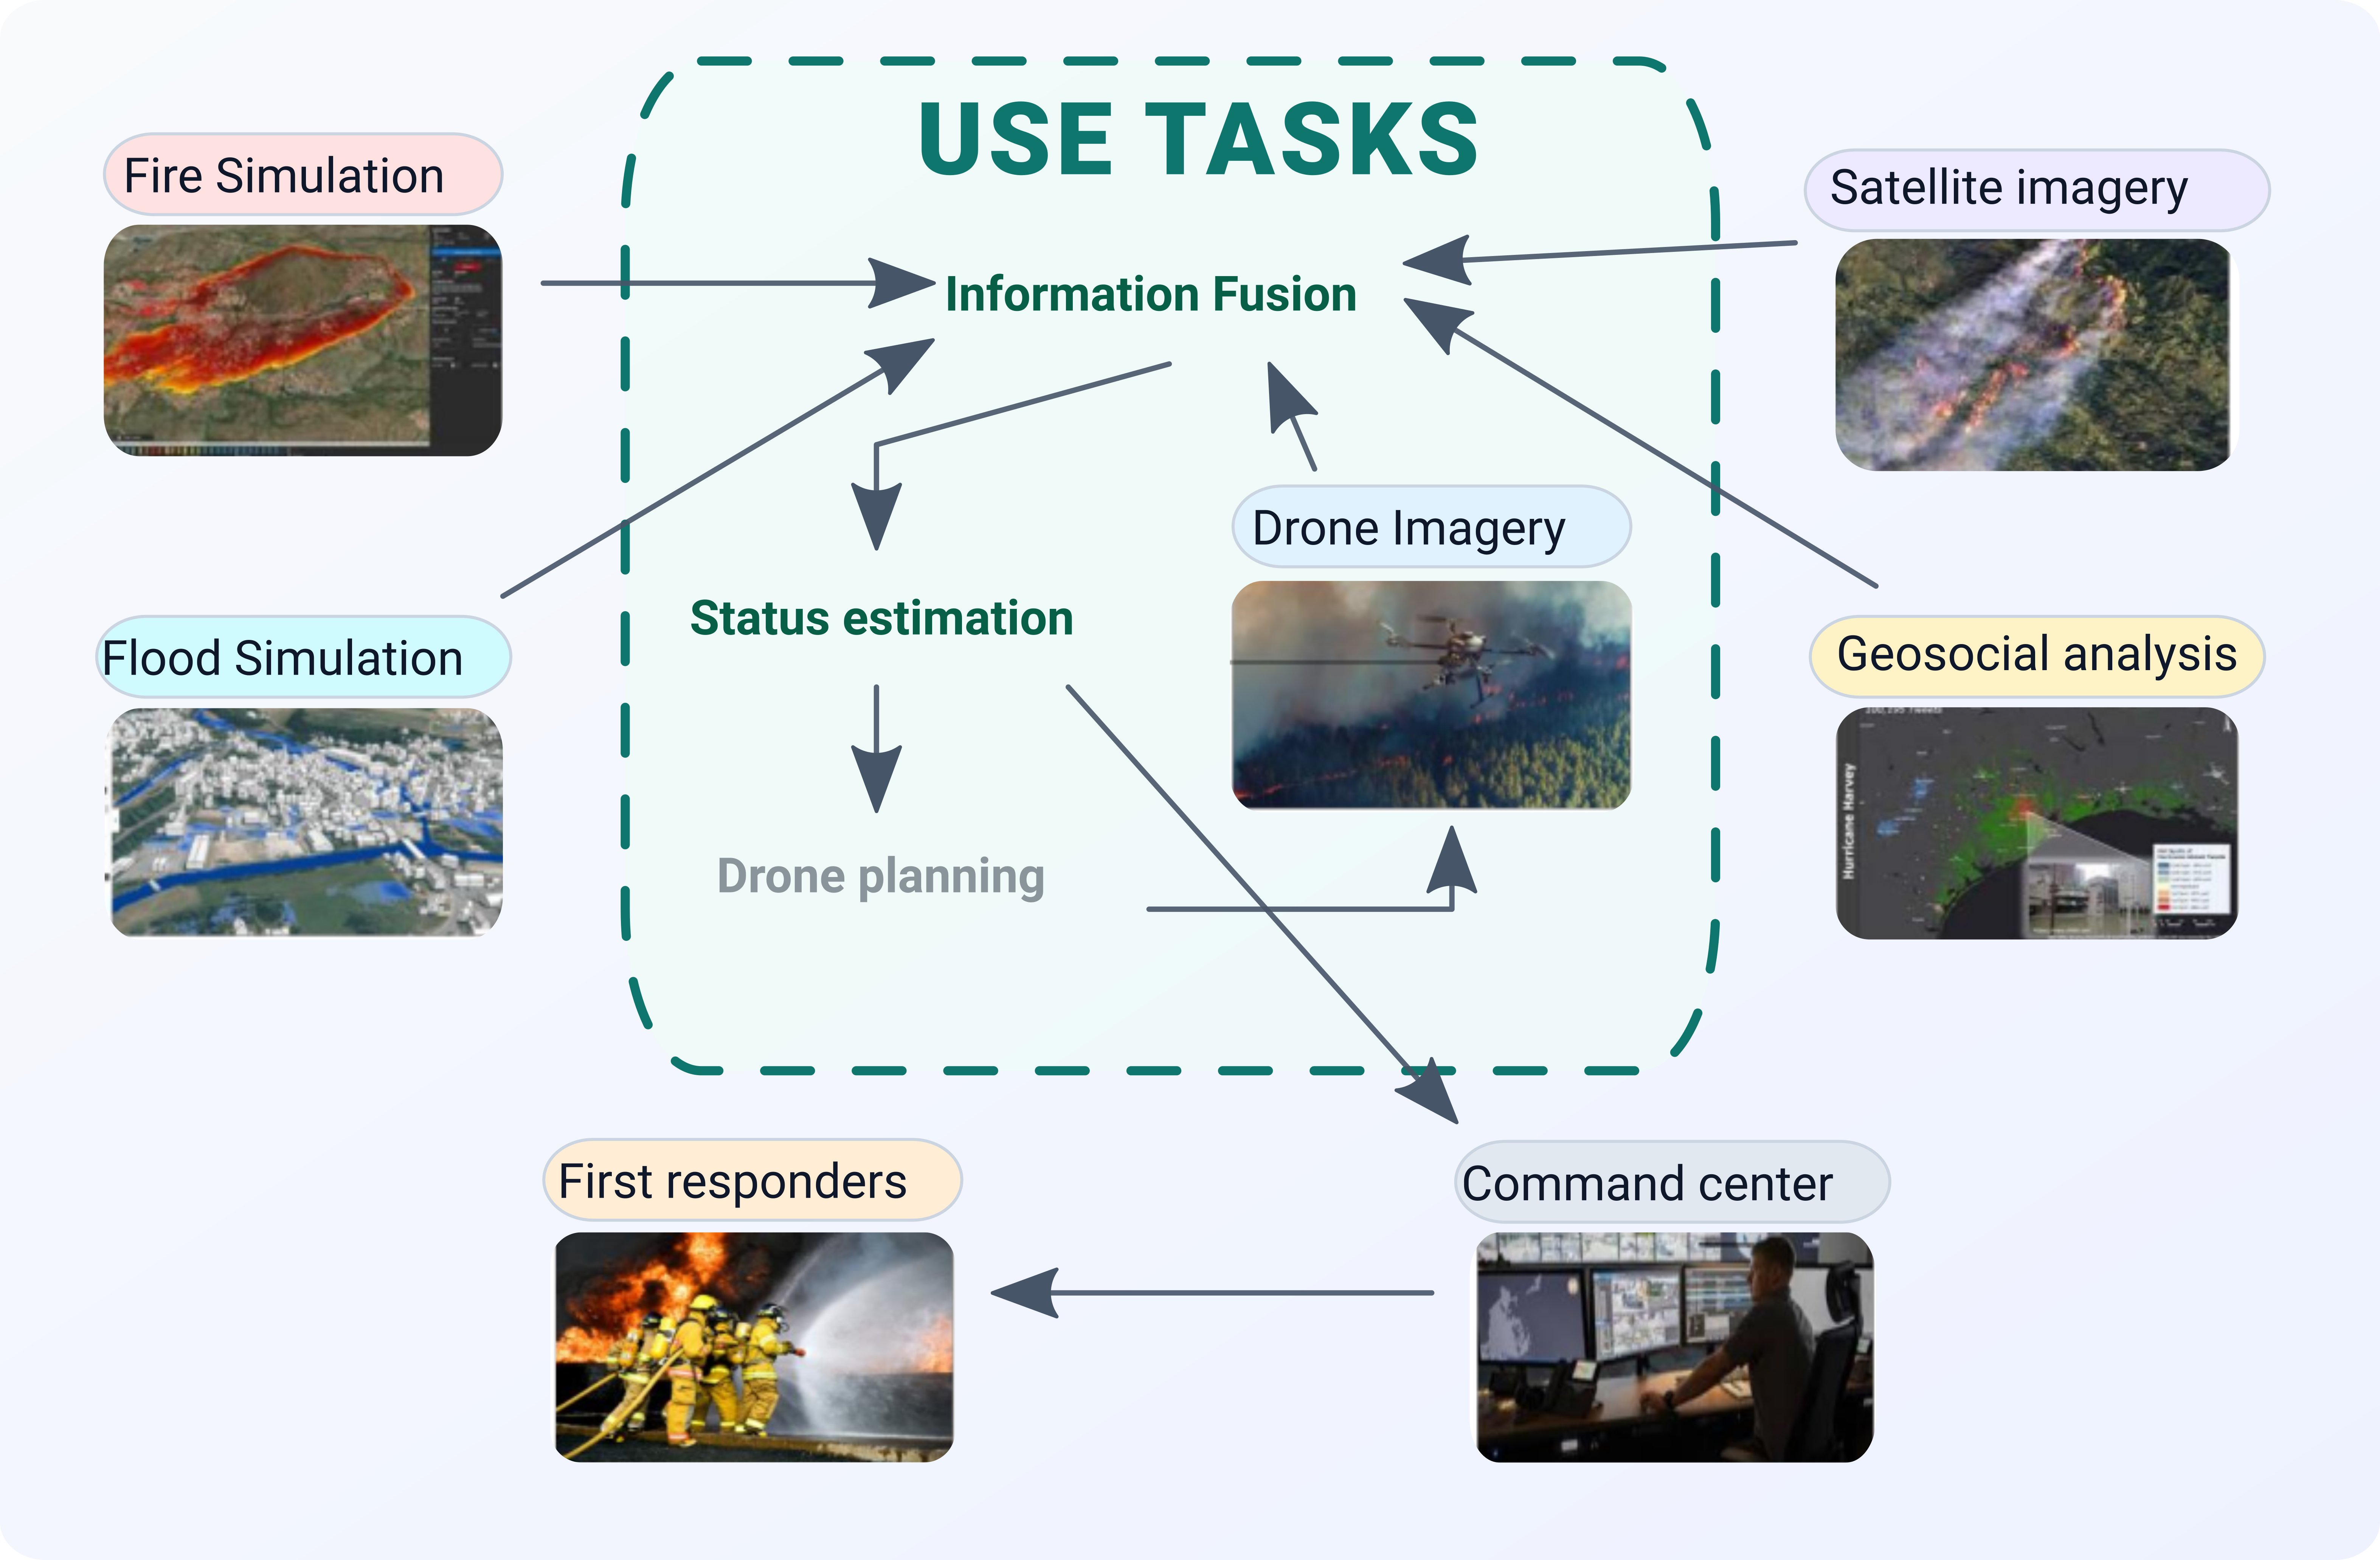
\includegraphics[
			width=\linewidth,
			height=0.62\textheight,
			keepaspectratio
			]{enhanced_end_to_end_scheme.png}
			
			\vspace{0.2em}
			{\scriptsize End-to-end workflow in TEMA.}
		\end{column}
	\end{columns}
	
\end{frame}


\begin{frame}{Key challenges addressed by PDM-tech-05}
  \begin{itemize}
    \item \textbf{Heterogeneity:} mixing observations (UAV/satellite/geosocial) with model predictions
    \item \textbf{Asynchrony:} data arrive at different times and rates; some regions are intermittently observed
    \item \textbf{Spatial mismatch:} different projections/resolutions \textrightarrow{} common reference grid
    \item \textbf{Uncertainty:} probabilistic representation + numerically stable updates (log-odds)
    \item \textbf{Scalability:} update only where data overlap AOI; event-driven processing
    \item \textbf{Actionability:} expose products via APIs and a web app to decision-support tools
  \end{itemize}
\end{frame}

\begin{frame}{What the Information Fusion platform does}
  \begin{columns}[T,onlytextwidth]
    \column{0.56\textwidth}
      \begin{block}{PDM-tech-05: generic fusion service for NDM}
        \begin{itemize}
          \item Select an Area of Interest (AOI) and a reference grid
          \item Ingest multi-modal streams with timestamps and georeferencing metadata
          \item Apply source-specific measurement/prediction models
          \item Maintain a persistent probabilistic state (\textbf{OGM} + \textbf{OPM})
          \item Serve updates to the Digital Enabler / SmartDesk and trigger workflows
        \end{itemize}
      \end{block}
    \column{0.40\textwidth}
      \begin{block}{Design principle}
        \textbf{Convert everything into consistent probabilities on a common spatial reference, then fuse.}
      \end{block}
  \end{columns}
\end{frame}

\begin{frame}{Two primary outputs: OGM and OPM}
  \begin{columns}[T,onlytextwidth]
    \column{0.49\textwidth}
      \begin{block}{1) Occupancy Grid Map (OGM)}
        \begin{itemize}
          \item Regular grid over AOI (e.g., 5 m cells)
          \item Each cell stores a hazard probability:
            \begin{itemize}
              \item \textit{Maps4Flood:} flood probability
              \item \textit{Maps4Fire:} fire/burnt probability
            \end{itemize}
          \item Updated asynchronously as new evidence arrives
        \end{itemize}
      \end{block}

    \column{0.49\textwidth}
      \begin{block}{2) Object Presence Map (OPM)}
        \begin{itemize}
          \item Tracks dynamic entities (persons / vehicles)
          \item Geodetic state with uncertainty (Kalman filtering)
          \item Data association (gating + Hungarian assignment)
          \item Supports responder-centric risk awareness
        \end{itemize}
      \end{block}
  \end{columns}
\end{frame}



\begin{frame}{How PDM-tech-05 connects to other TEMA technologies}
  \centering
  \includegraphics[width=0.98\linewidth,height=0.80\textheight,keepaspectratio]{INTERACTION_DIAGRAM.png}
\end{frame}

\begin{frame}{Web app and services architecture (deployment view)}
  \centering
  \includegraphics[width=0.95\linewidth,height=0.750\textheight,keepaspectratio]{web_app_diagram.png}
\end{frame}

\begin{frame}{Core engine: asynchronous occupancy-grid mapping}
  \begin{columns}[T,onlytextwidth]
    \column{0.55\textwidth}
      \begin{itemize}
        \item Maintain a grid of \textbf{log-odds} values (numerically stable)
        \item \textbf{Correction (sensor fusion):} apply an update when a new measurement arrives
        \item \textbf{Prediction (model-based):} propagate using predictions when measurements are absent
        \item Event-driven: each source triggers only the relevant update on overlapping cells
      \end{itemize}
    \column{0.43\textwidth}
      \centering
      \includegraphics[width=\linewidth,height=0.66\textheight,keepaspectratio]{asyncapproach.png}
  \end{columns}
\end{frame}

\begin{frame}{OGM formalism: probability and log-odds}
  \scriptsize
  \begin{block}{Occupancy grid cell $m_i$ (hazard present vs. absent)}
    Posterior occupancy probability after fusing measurements up to time $t$:
    \[
      p^t_i = P(m_i \mid z_{1:t}, x_{1:t}), \qquad
      \ell^t_i = \log\frac{p^t_i}{1-p^t_i}.
    \]
    With a prior $p^0_i=P(m_i)$, the initial log-odds is
    \[
      \ell^0_i = \log\frac{p^0_i}{1-p^0_i}.
    \]
  \end{block}

  \vspace{-0.8em}
  \begin{block}{Update in log-odds space (Bayesian occupancy update)}
    Each new, georeferenced measurement contributes an additive increment:
    \[
      \ell^{t}_i = \ell^{t-}_i + \delta\ell^{t}_{i,s}, \qquad
      \delta\ell^{t}_{i,s} = \log\frac{p^{t}_{i,s}}{1-p^{t}_{i,s}},
    \]
    followed by the inverse logistic map $p^{t}_i = \sigma(\ell^{t}_i)=\bigl(1+e^{-\ell^{t}_i}\bigr)^{-1}$.
  \end{block}
\end{frame}

\begin{frame}{Fusion rule: measurements vs. predictions}
  \begin{columns}[T,onlytextwidth]
    \column{0.54\textwidth}
      \begin{block}{Observational sources (UAV / satellite / geosocial)}
        \begin{itemize}
          \item Convert raw outputs into a per-cell probability $p^{t}_{i,s}\in(0,1)$
          \item Add a log-odds increment $\delta\ell^{t}_{i,s} = \log\frac{p^{t}_{i,s}}{1-p^{t}_{i,s}}$
          \item Intuition: \textbf{high-confidence observations dominate locally}
        \end{itemize}
      \end{block}
    \column{0.42\textwidth}
      \begin{block}{Predictive sources (models)}
        \begin{itemize}
          \item Predictions provide \textbf{structured early evidence} over large areas
          \item Fuse with the current OGM via \textbf{logit pooling} (weighted combination in log-odds space)
          \item Intuition: \textbf{predictions guide} until observations override
        \end{itemize}
      \end{block}
  \end{columns}
\end{frame}

\begin{frame}{Flood measurement model: UAV flood segmentation (TFA-tech-06)}
  \scriptsize
  \begin{block}{Aggregation from high-resolution UAV raster to the OGM grid}
    For cell $i$, let $K_i$ be the set of georeferenced UAV pixels inside $i$ and $n_i=|K_i|$.
    The aggregated score is
    \[
      \bar{s}^{\text{uav}}_i=\frac{1}{n_i}\sum_{k\in K_i} s^{\text{uav}}_k \in [0,1].
    \]
    Map the score to a measurement probability
    \[
      p^{\text{uav}}_i = p^{\text{uav}}_{\min} + \bigl(p^{\text{uav}}_{\max}-p^{\text{uav}}_{\min}\bigr)\,\bar{s}^{\text{uav}}_i,
      \qquad 0<p^{\text{uav}}_{\min}<p^{\text{uav}}_{\max}<1,
    \]
    then apply the additive log-odds update $\delta\ell^{t}_{i,\text{uav}}=\log\frac{p^{\text{uav}}_i}{1-p^{\text{uav}}_i}$.
  \end{block}
\end{frame}

\begin{frame}{Flood measurement model: satellite flood extent (TFA-tech-08)}
  \scriptsize
  \begin{block}{Per-cell probability from a resampled satellite mask}
    Let $m^{\text{sat}}_i\in[0,1]$ be the resampled satellite mask value at cell $i$.
    For valid pixels:
    \[
      p^{\text{sat}}_i = m^{\text{sat}}_i \in (0,1),
      \qquad
      \delta\ell^{t}_{i,\text{sat}} = \log\frac{p^{\text{sat}}_i}{1-p^{\text{sat}}_i}.
    \]
    Cells outside the satellite swath (or invalid pixels) are not updated.
  \end{block}
  \vspace{-0.4em}
  \begin{block}{Implementation note}
    Probabilities are clamped to $[\epsilon,1-\epsilon]$ (e.g., $\epsilon\approx 10^{-6}$) to avoid infinite log-odds.
  \end{block}
\end{frame}

\begin{frame}{Flood measurement model: geosocial hotspots (TFA-tech-11)}
  \scriptsize
  \begin{block}{From counts/ratios to measurement probability}
    Let $\tilde{c}_t(i)$ and $\tilde{r}_t(i)$ be normalized post count and activity ratio, and $w_c+w_r=1$.
    Define a hotspot score
    \[
      s^{\text{soc}}_t(i)=w_c\,\tilde{c}_t(i)+w_r\,\tilde{r}_t(i)\in[0,1],
    \]
    then convert to a probability
    \[
      p^{\text{soc}}_t(i)=\epsilon + (1-2\epsilon)\,s^{\text{soc}}_t(i),
      \qquad
      \delta\ell^{t}_{i,\text{soc}} = \log\frac{p^{\text{soc}}_t(i)}{1-p^{\text{soc}}_t(i)}.
    \]
  \end{block}
  \vspace{-0.4em}
  \begin{block}{Interpretation}
    Geosocial evidence is informative but noisy; weights are typically conservative compared to physical sources.
  \end{block}
\end{frame}

\begin{frame}{Flood prediction fusion: hydrodynamic depth (PDM-tech-02 / 3Di)}
  \scriptsize
  \begin{block}{Depth-to-probability mapping (soft evidence)}
    For a predicted water depth $h_i\ge 0$, define
    \[
      p^{\text{hyd}}_i=\epsilon+(1-2\epsilon)\,\frac{1}{1+\exp\!\bigl(-(h_i-h_{50})/s\bigr)}.
    \]
  \end{block}
  \vspace{-0.6em}
  \begin{block}{Logit pooling with the current map state}
    Convert to log-odds $\ell^{\text{ogm}}_i=\log\frac{p^{\text{ogm}}_i}{1-p^{\text{ogm}}_i}$ and
    $\ell^{\text{hyd}}_i=\log\frac{p^{\text{hyd}}_i}{1-p^{\text{hyd}}_i}$, then fuse:
    \[
      \ell^{\text{new}}_i=(1-\alpha_{\text{hyd}})\,\ell^{\text{ogm}}_i + \alpha_{\text{hyd}}\,\ell^{\text{hyd}}_i,
      \qquad
      p^{\text{new}}_i=\sigma(\ell^{\text{new}}_i).
    \]
  \end{block}
\end{frame}

\begin{frame}{Fusing predictive outputs in a generic way}
  \scriptsize
  \begin{block}{Prediction as probabilistic evidence (example: fire arrival / flood simulation)}
    For cell $i$, represent prediction as a pair of probabilities (hazard / no hazard):
    \[
      p^{\text{pred}}_i
      = \frac{w_f\,p_f(i) + w_{nf}\,p_{nf}(i)}{w_f+w_{nf}},
      \qquad w_f,w_{nf}>0.
    \]
    \vspace{-0.5em}
    \begin{itemize}
      \item \textbf{Flood:} $p_f(i)$ from model-derived inundation probability; $p_{nf}(i)=1-p_f(i)$.
      \item \textbf{Fire:} $p_f(i)$ from arrival-time evidence (e.g., within a forecast horizon); $p_{nf}(i)=1-p_f(i)$.
    \end{itemize}
  \end{block}
  \vspace{-0.6em}
  \begin{block}{How it enters the OGM}
    Use the same update interface as observations: convert $p^{\text{pred}}_i$ to log-odds and fuse
    (typically via logit pooling to reflect its ``prior-like'' role).
  \end{block}
\end{frame}

\begin{frame}{Extending beyond floods: fire occupancy (Maps4Fire)}
  \scriptsize
  \begin{block}{Fire-related measurements (examples)}
    \begin{itemize}
      \item UAV: \textit{FireSegmentation} and \textit{BurntSegmentation} (TFA-tech-06)
      \item Satellite: \textit{EOBurntArea} (TFA-tech-09)
      \item Geosocial: \textit{HotspotResult} (TFA-tech-11)
      \item Prediction: \textit{StandardArrivalTime} (PDM-tech-01)
    \end{itemize}
  \end{block}
  \vspace{-0.6em}
  \begin{block}{Example weighted combination (active fire vs. burnt evidence)}
    \[
      p_m(m_i)=w_{\text{fire}}\,p_{\text{fire}}(m_i)+w_{\text{burnt}}\,p_{\text{burnt}}(m_i),
      \qquad w_{\text{fire}}+w_{\text{burnt}}=1.
    \]
    This per-cell likelihood plugs into the same Bayesian occupancy update in log-odds space.
  \end{block}
\end{frame}

\begin{frame}{OPM: state, motion model, and asynchronous updates}
  \scriptsize
  \begin{block}{Geodetic state for each tracked object $k$}
    \[
      \mathbf{x}_{t,k}=\bigl[\lambda_{t,k}\;\;\phi_{t,k}\;\;h_{t,k}\;\;\dot{\lambda}_{t,k}\;\;\dot{\phi}_{t,k}\;\;\dot{h}_{t,k}\bigr]^{\top}.
    \]
  \end{block}
  \vspace{-0.6em}
  \begin{block}{Constant-velocity prediction (discrete time)}
    \[
      \hat{\mathbf{x}}_{t|t-1,k}=A_t\,\hat{\mathbf{x}}_{t-1|t-1,k},
      \qquad
      P_{t|t-1,k}=A_t\,P_{t-1|t-1,k}\,A_t^{\top}+R_t.
    \]
  \end{block}
  \vspace{-0.6em}
  \begin{block}{Rationale}
    Tracks persist even when detections are intermittent; uncertainty grows during prediction-only periods.
  \end{block}
\end{frame}

\begin{frame}{OPM: correction and data association}  
  \begin{columns}[T,onlytextwidth]
    \column{0.52\textwidth}
    \tiny
      \begin{block}{Kalman correction (when detection $z_{t,j}$ is assigned)}
        \[
          S_{t,j,k}=H P_{t|t-1,k}H^{\top}+R_{t,j},
          \quad
          K_{t,j,k}=P_{t|t-1,k}H^{\top}S^{-1}_{t,j,k},
        \]
        \[
          \hat{\mathbf{x}}_{t|t,k}=\hat{\mathbf{x}}_{t|t-1,k}
          +K_{t,j,k}\bigl(z_{t,j}-H\hat{\mathbf{x}}_{t|t-1,k}\bigr),
          \quad
          P_{t|t,k}=(I-K_{t,j,k}H)P_{t|t-1,k}.
        \]
      \end{block}

    \column{0.46\textwidth}
      \begin{block}{Association: gating + Hungarian}
        \begin{itemize}
          \item Gate candidates by geodetic distance (e.g., haversine) within $r_{\text{gate}}$
          \item Solve a minimum-cost assignment with cost
            \[
              C_{k,j}=\alpha\,\frac{d_{\text{hav}}(\hat{p}_{t|t-1,k},p_{t,j})}{r_{\text{gate}}}
              +\beta\,(1-c^{\text{det}}_{t,j}).
            \]
        \end{itemize}
      \end{block}
  \end{columns}
\end{frame}

\begin{frame}{Case study focus: floods (Ahrtal) as a demonstrator}
  \begin{block}{Why a flood case study?}
    The platform is hazard-agnostic, but floods provide a clear demonstration of fusing
    predictions (hydrodynamics) with heterogeneous observations (UAV, satellite, geosocial).
  \end{block}

  \vspace{-0.2em}
  \begin{itemize}
    \item AOI defined as a polygon; OGM grid initialised with $p_i=0.5$ (unknown)
    \item Sources fused asynchronously upon arrival:
      \begin{itemize}
        \item 3Di depth predictions \textrightarrow{} soft prior via logit pooling
        \item UAV flood segmentation \textrightarrow{} high-resolution local corrections
        \item Satellite flood extent \textrightarrow{} broader-area observational updates
        \item Geosocial hotspots \textrightarrow{} human-centric weak evidence
      \end{itemize}
    \item Outputs delivered to decision-support tools: OGM (flood status) + OPM (persons/vehicles)
  \end{itemize}
\end{frame}

\begin{frame}{Key takeaways}
  \begin{itemize}
    \item \textbf{Generic platform:} one fusion engine, multiple hazards (floods, wildfires, \dots)
    \item \textbf{Two operational products:} OGM for hazard status; OPM for dynamic entities
    \item \textbf{Robust fusion:} log-odds updates for observations + logit pooling for predictions
    \item \textbf{System-ready:} deployed as web services with APIs and a web app
    \item \textbf{USE contribution:} PDM-tech-05 (fusion) integrated with UAV acquisition and drone planning
  \end{itemize}
\end{frame}





\begin{frame}{Frame Title}
    
\end{frame}

\begin{frame}{Frame Title}
    
\end{frame}

\begin{frame}{Frame Title}
    
\end{frame}

\begin{frame}{Frame Title}
    
\end{frame}

\begin{frame}{Frame Title}
    
\end{frame}

\begin{frame}{Frame Title}
    
\end{frame}

\begin{frame}{Frame Title}
    
\end{frame}

\begin{frame}{Frame Title}
    
\end{frame}

\begin{frame}{Frame Title}
    
\end{frame}

\begin{frame}{Frame Title}
    
\end{frame}

\begin{frame}{Frame Title}
    
\end{frame}

\begin{frame}{Frame Title}
    
\end{frame}

\begin{frame}{Frame Title}
    
\end{frame}

\begin{frame}{Frame Title}
    
\end{frame}

\end{document}
